We used the Pima Indians Diabetes Dataset from the National Institute of Diabetes and Digestive and Kidney Diseases. This dataset has a binary response variable indicating if the sample has diabetes and eight covariates on 768 samples. The data was standardized to have mean zero and standard deviation one. As discussed above, the parameters need to be chosen with care or the algorithm will mix poorly. \\

We can see that using the Hamiltonian Monte Carlo algorithm produced good mixing with energy decreasing downwards and converging. This means the sampling algorithm is spending most of its time in states of higher posterior probability.

\begin{figure}[H]
	\centering
	\begin{minipage}{0.45\textwidth}
		\centering
		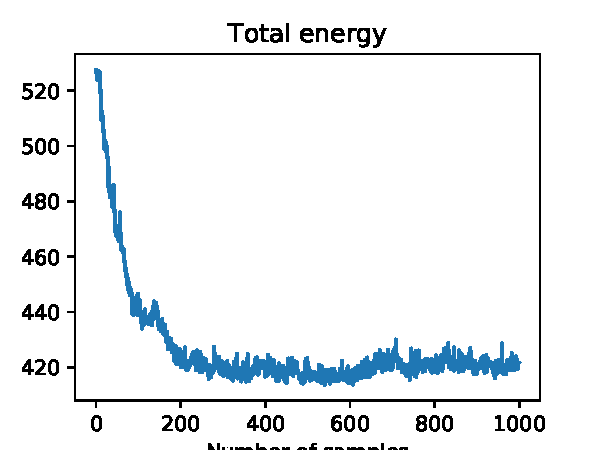
\includegraphics[width=0.9\textwidth]{hmc-energy-pima.pdf} % first figure itself
	\end{minipage}\hfill
	\begin{minipage}{0.45\textwidth}
		\centering
		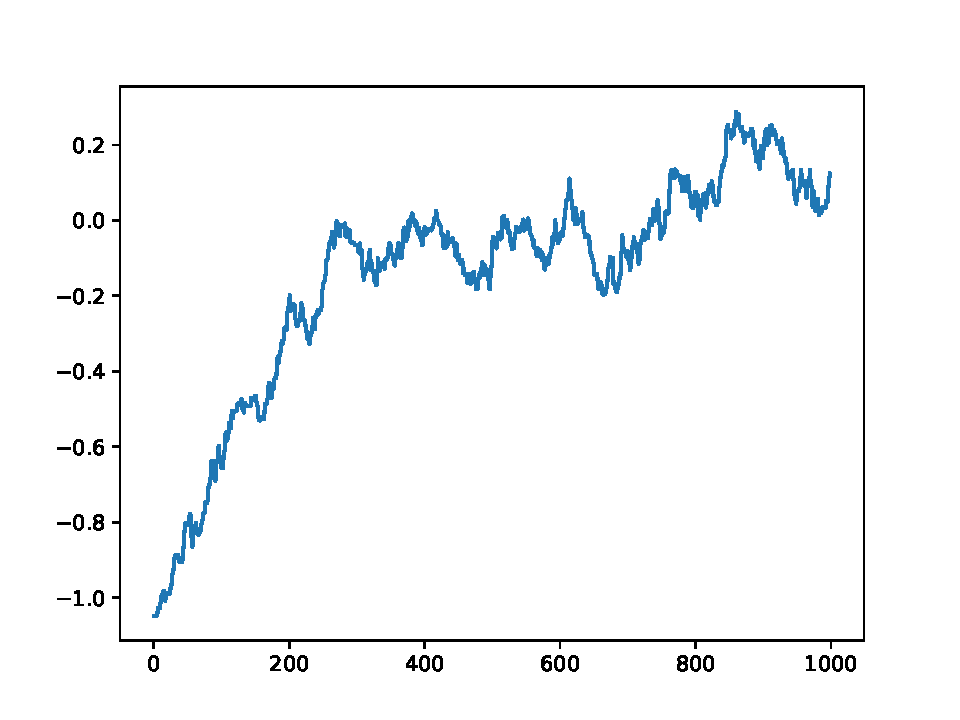
\includegraphics[width=0.9\textwidth]{hmc-trace-pima.pdf} % second figure itself
	\end{minipage}
\end{figure}

We can see that using the Stochastic Gradient Hamiltonian Monte Carlo algorithm produced good mixing with energy decreasing downwards and converging:

\begin{figure}[H]
	\centering
	\begin{minipage}{0.45\textwidth}
		\centering
		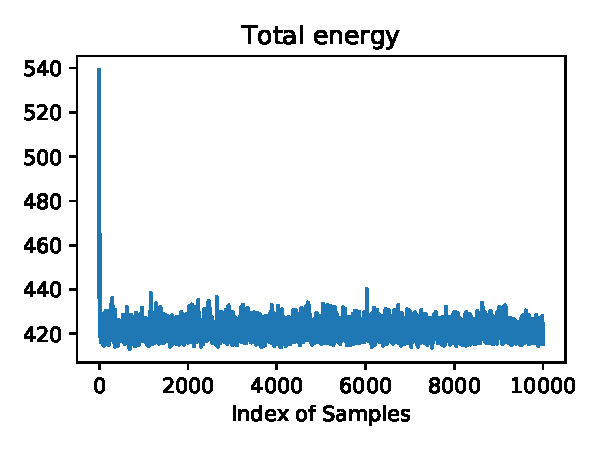
\includegraphics[width=0.9\textwidth]{sghmc-energy-pima.pdf} % first figure itself
	\end{minipage}\hfill
	\begin{minipage}{0.45\textwidth}
		\centering
		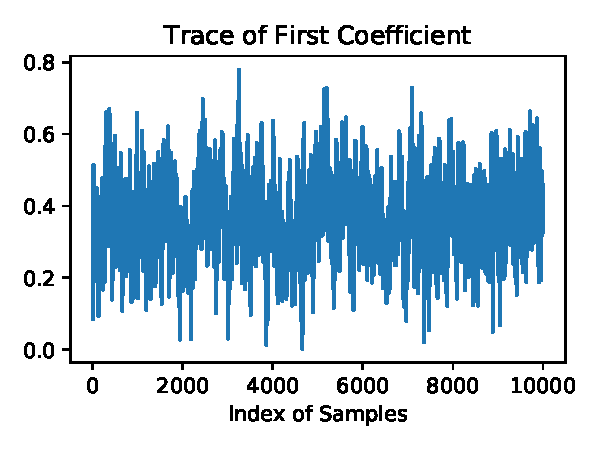
\includegraphics[width=0.9\textwidth]{sghmc-trace-pima.pdf} % second figure itself
	\end{minipage}
\end{figure}


We compared the coefficients produced by each algorithm to the MLE estimates to check for accuracy:

\begin{figure}[H]
	\centering
	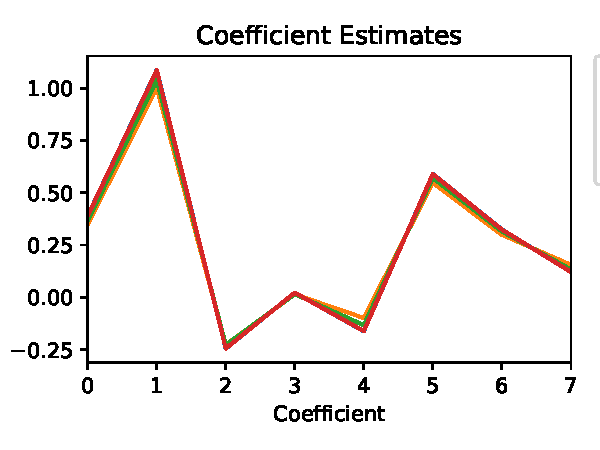
\includegraphics[width=0.45\textwidth]{coefs-pima.pdf}
\end{figure}

We see that all coefficients are similar.